%\documentclass[a4paper,oneside,onecolumn]{article}
\documentclass[journal=nalefd,manuscript=letter]{achemso}
\usepackage{graphicx}
\usepackage{amsmath}
\usepackage{amssymb}
\usepackage{subfigure}
%\usepackage{epstopdf}
%\usepackage{setspace}
%\onehalfspace
%\usepackage{authblk}
%\usepackage[margin=2.3cm]{geometry}

%\geometry{a4paper,left=2.3cm,right=2.3cm,top=2.5cm,bottom=4.5cm}

\usepackage[version=3]{mhchem} % Formula subscripts using \ce{}
\usepackage[T1]{fontenc}       % Use modern font encodings
\renewcommand{\thefigure}{S\arabic{figure}}%
\newcommand{\nm}{\ensuremath{\,\textrm{nm}}}
\newcommand{\um}{\ensuremath{\,\mu\textrm{m}}}
\newcommand{\eV}{\ensuremath{\,\textrm{eV}}}
\newcommand{\uM}{\ensuremath{\,\mu\textrm{M}}}
\newcommand{\uW}{\ensuremath{\,\mu\textrm{W}}}
\newcommand{\meV}{\ensuremath{\,\textrm{meV}}}
\newcommand{\pwr}{\ensuremath{\,\textrm{kW/cm}^2}}
\newcommand{\CPS}{\ensuremath{\,\textrm{cps}}}
\newcommand{\atto}{\ensuremath{\textrm{ATTO}\,647\textrm{N}}}

\author{Aquiles Carattino}
\affiliation[Leiden]
{Huygens-Kamerlingh Onnes, Leiden, The Netherlands}
\author{Veer Keizer}
\affiliation[Leiden]
{Huygens-Kamerlingh Onnes, Leiden, The Netherlands}
\author{Marcel Schaaf}
\affiliation[Leiden]
{Huygens-Kamerlingh Onnes, Leiden, The Netherlands}
\author{Michel Orrit}
\email{orrit@physics.leidenuniv.nl}
\affiliation[Leiden]
{Huygens-Kamerlingh Onnes Lab, 2300RA Leiden, The Netherlands}

\title{Supplementary Information for: Background-free imaging of gold nanorods
through detection of anti-Stokes emission}

\keywords{Gold nanorods, Plasmon, Imaging, Anti-Stokes, Bio-imaging, Confocal}

\begin{document}
\maketitle
\abstract{This is the abstract}


\section{Setup}

\begin{figure}[htp]
 \centering
 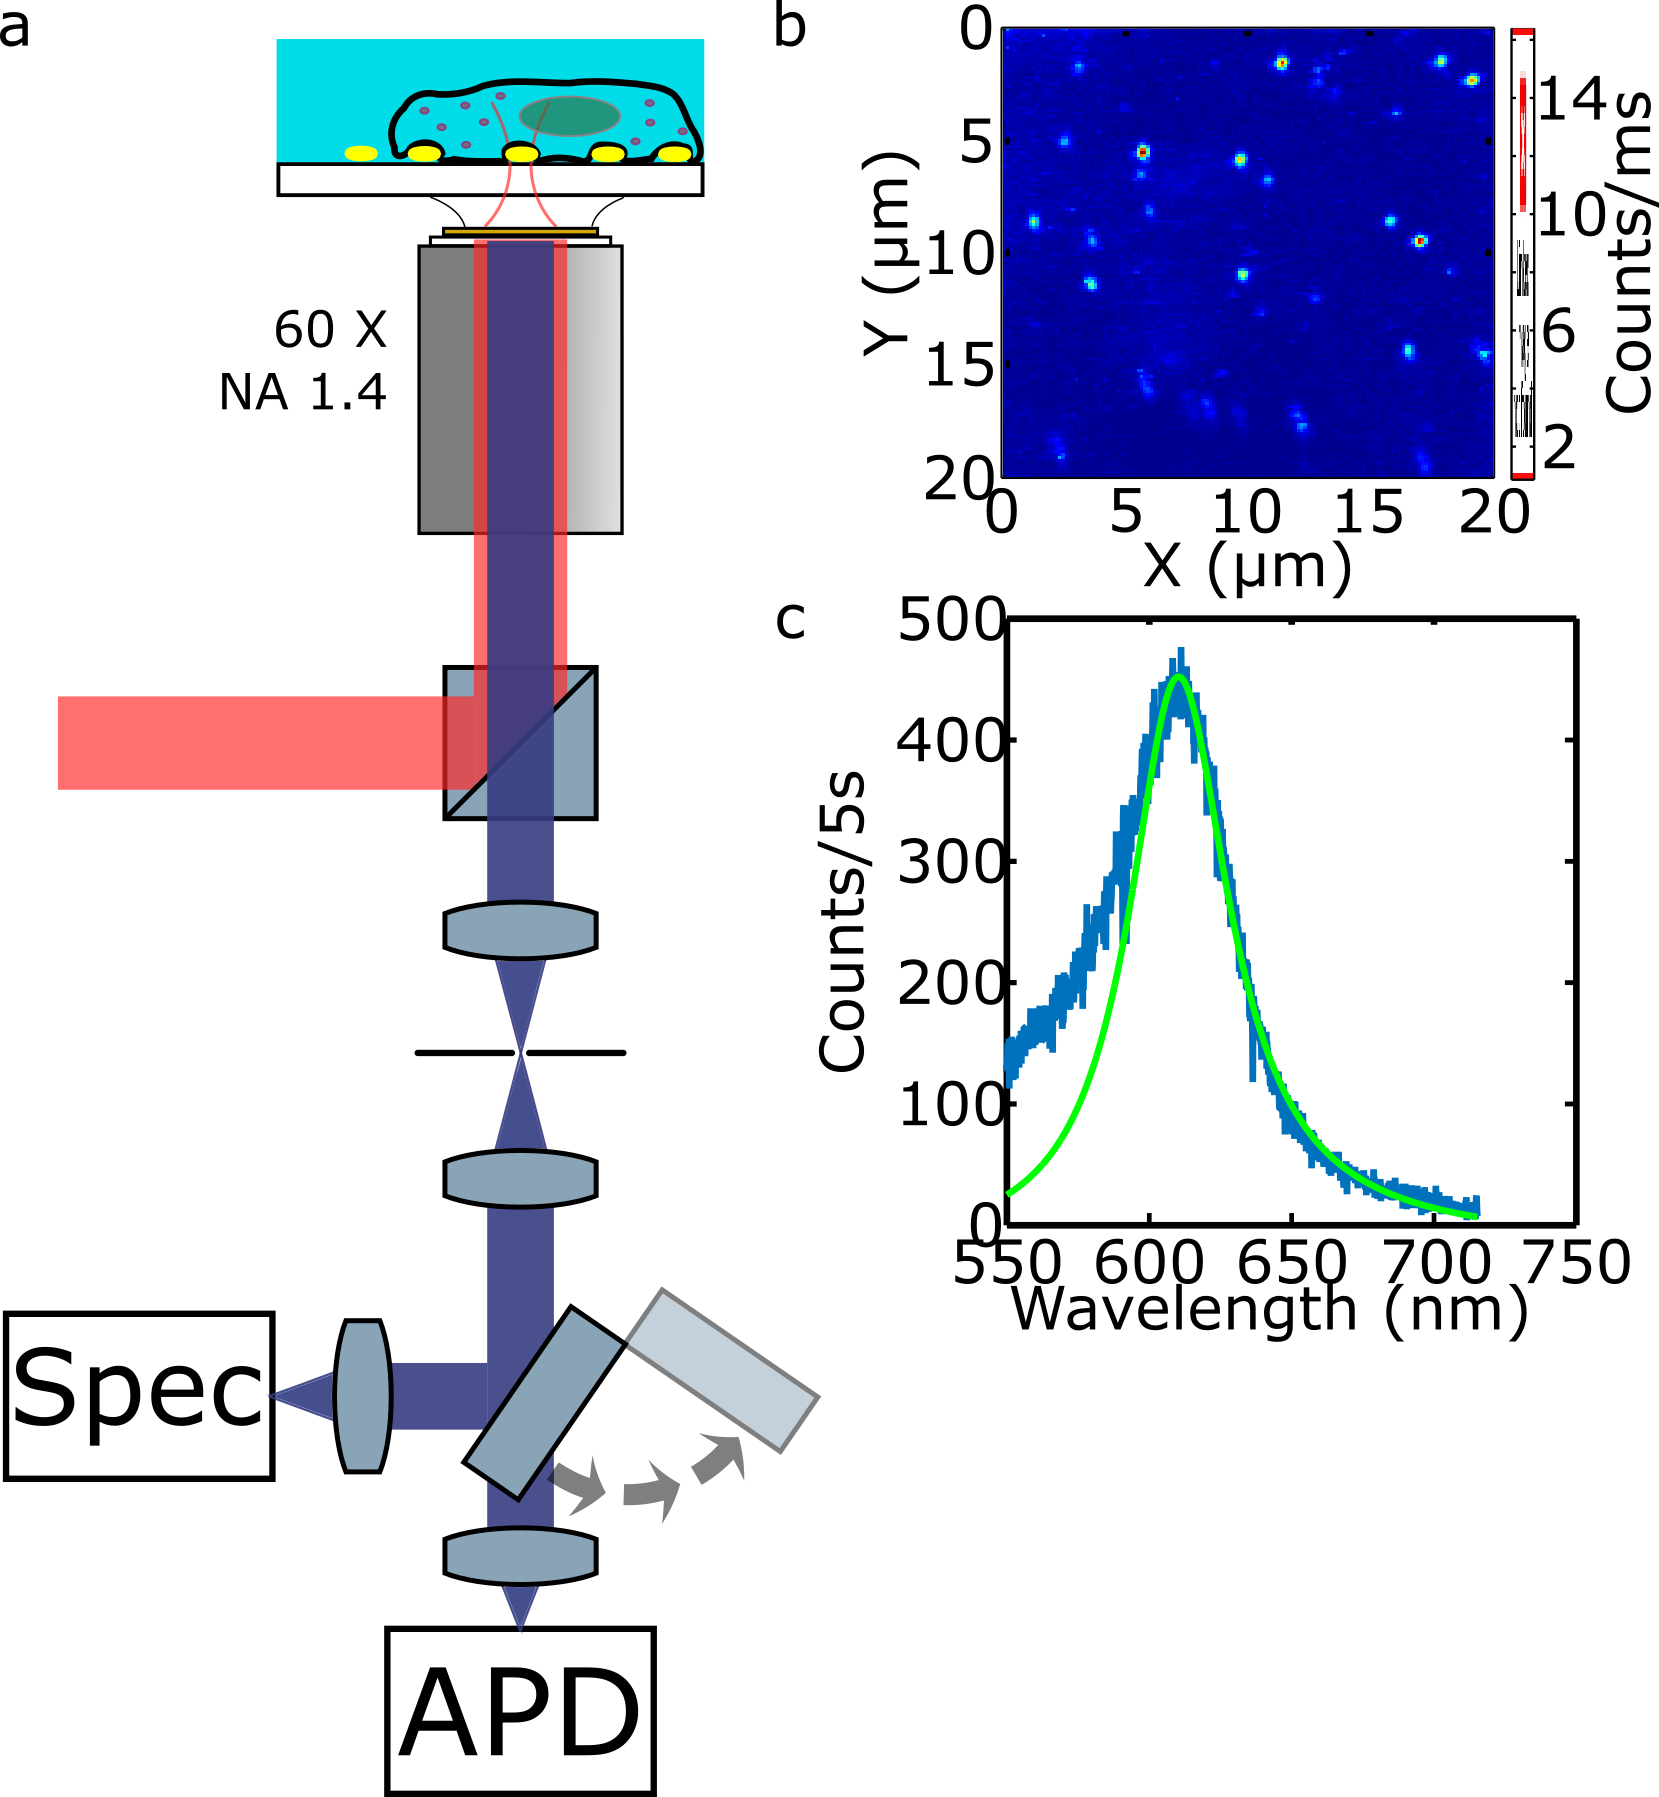
\includegraphics[width=0.45\textwidth]{Figures/Supplementary/01_Setup/setup_1.png}
 \caption{Experimental setup and examples of observations. a) Simplified
 schematic of the confocal microscope employed during the measurements. b) A
 typical 1-photon luminescence raster scan of the sample immersed in water c)
 luminescence spectrum of a single rod.}
 \label{fig:setup}
\end{figure}

Figure \ref{fig:setup} shows the schematic of the confocal microscope employed
in the experiments. It is important to note the presence of a $50/50$
beamsplitter before the objective. Exchanging it for an appropriate dichroic
mirror would increase the collection efficiency. In this work we chose not to do
it because the beamsplitter allows to collect both the full emission under
$532\nm$ excitation and the Stokes/anti-Stokes emission under $633\nm$ without
changes in the optical path. 

\section{Uv-Vis spectrum}

\begin{figure}[htp]
 \centering
 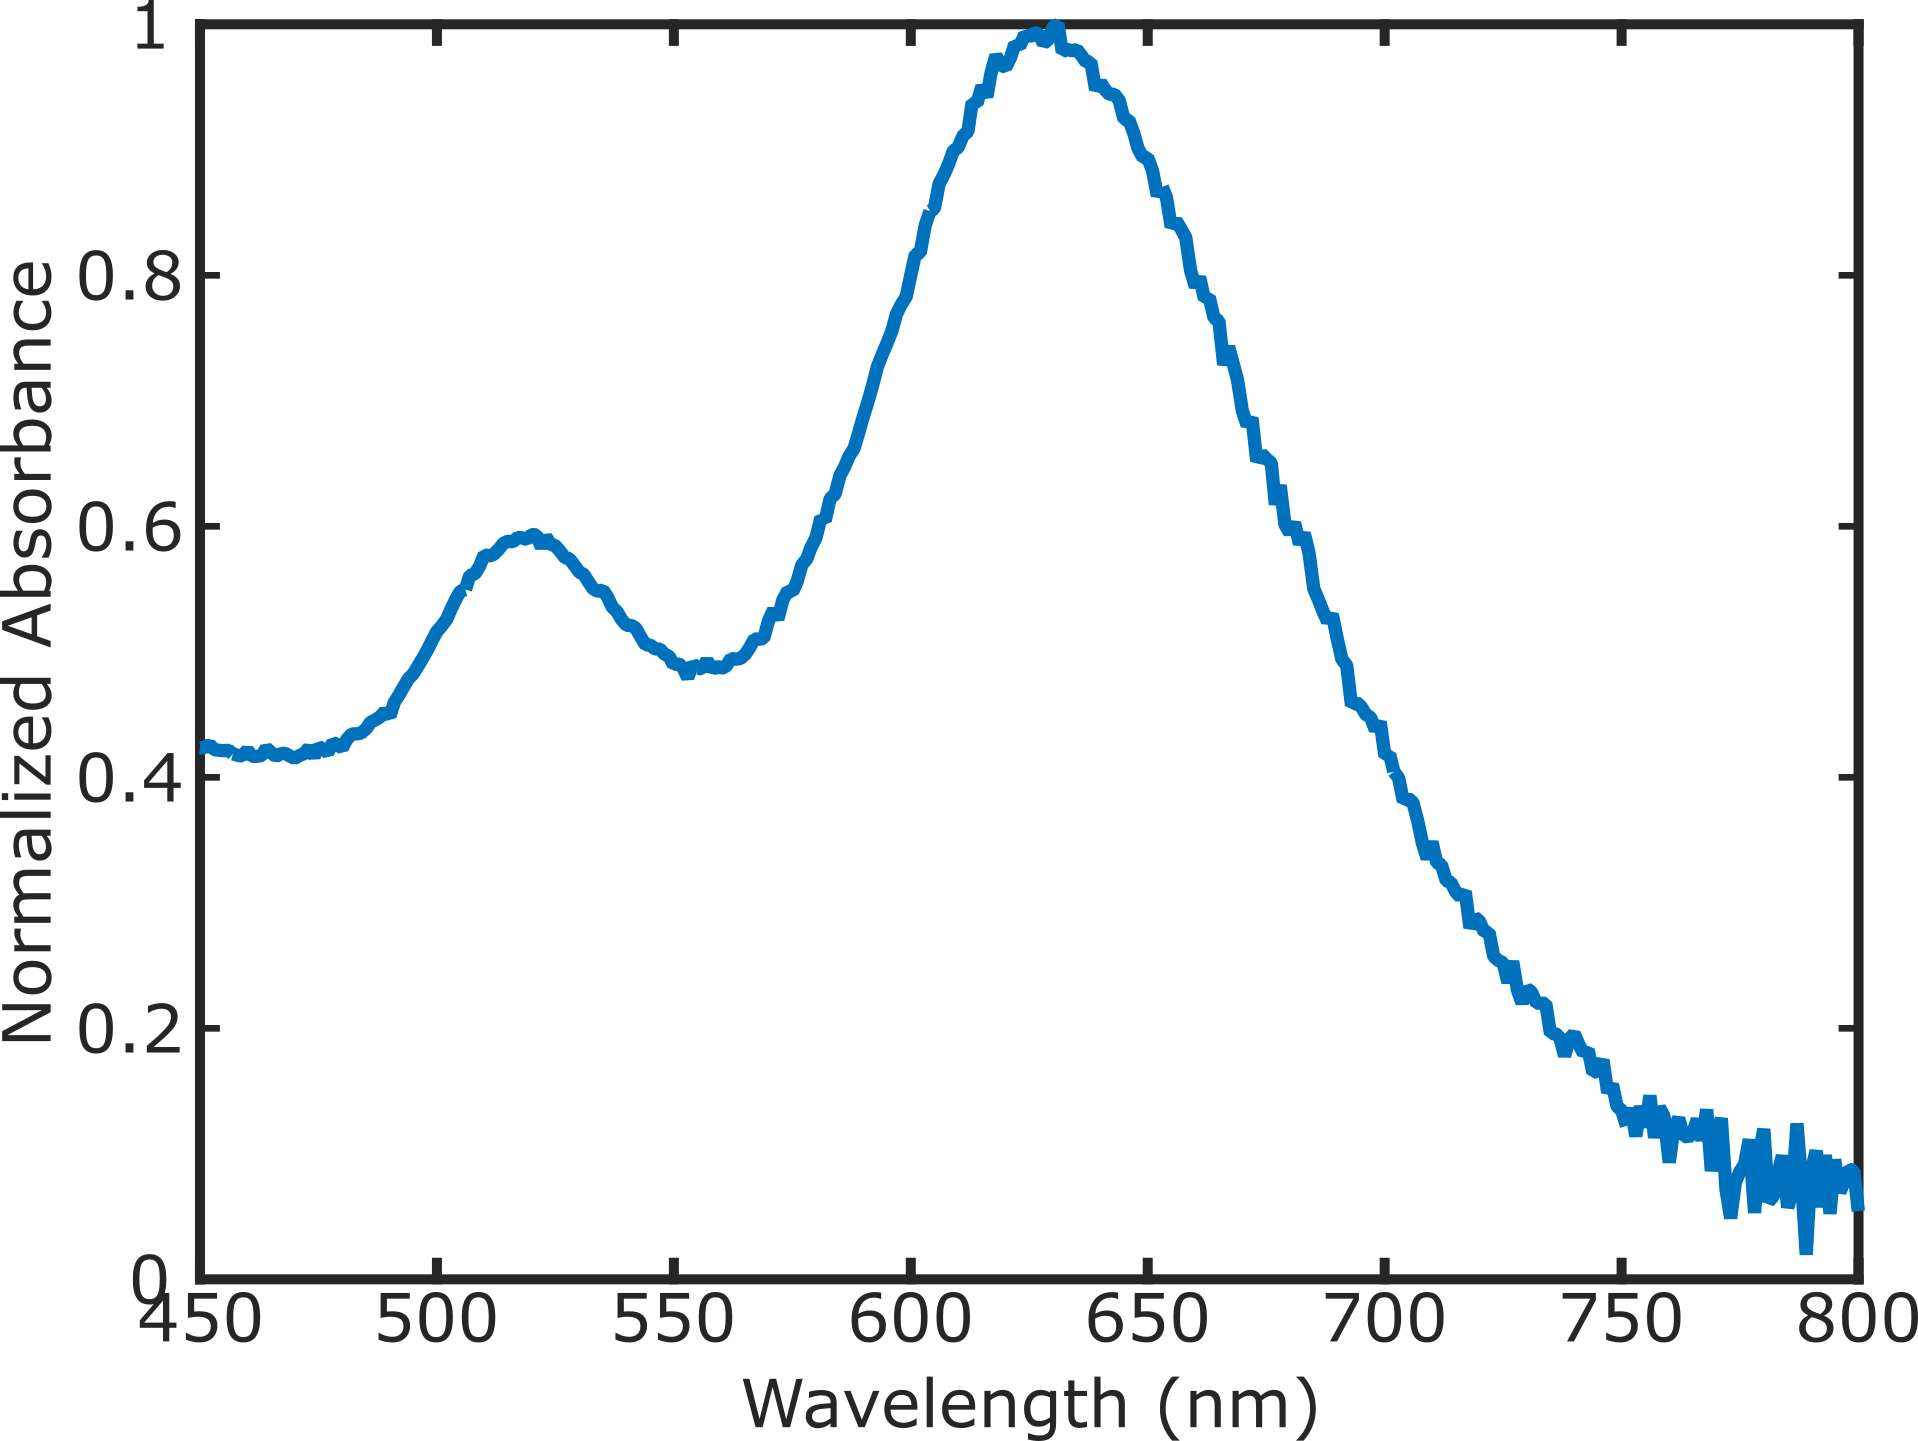
\includegraphics[width=0.45\textwidth]{Figures/Supplementary/02_UV-Vis/uvvis.png}
 \caption{Normalized extinction spectrum of a suspension of nanorods after
 synthesis. The resonance maximum is located at $630\nm$.}
 \label{fig:uvvis}
 \end{figure}
 
 Figure \ref{fig:uvvis} shows the extinction spectrum of the nanorod samples
 used throughout this work. Two peaks are clearly distinguishable, one around
 $630\nm$ that corresponds to the longitudinal plasmon resonance (LPR) of
 particles with sizes $25\nm\times50\nm$ and a second one at around $520\nm$.
 This peak normally corresponds to the presence of spheres as a by-product of the
 synthesis of the rods. The transverse plasmon resonance is also located at the
 same wavelength but is much weaker than the LPR. In a sample consisting of
 exclusively rods, the transverse resonance wouldn't be observable in an UV-Vis
 spectrometer.
 
 \section{Filters}

\begin{figure}[htp]
 \centering
 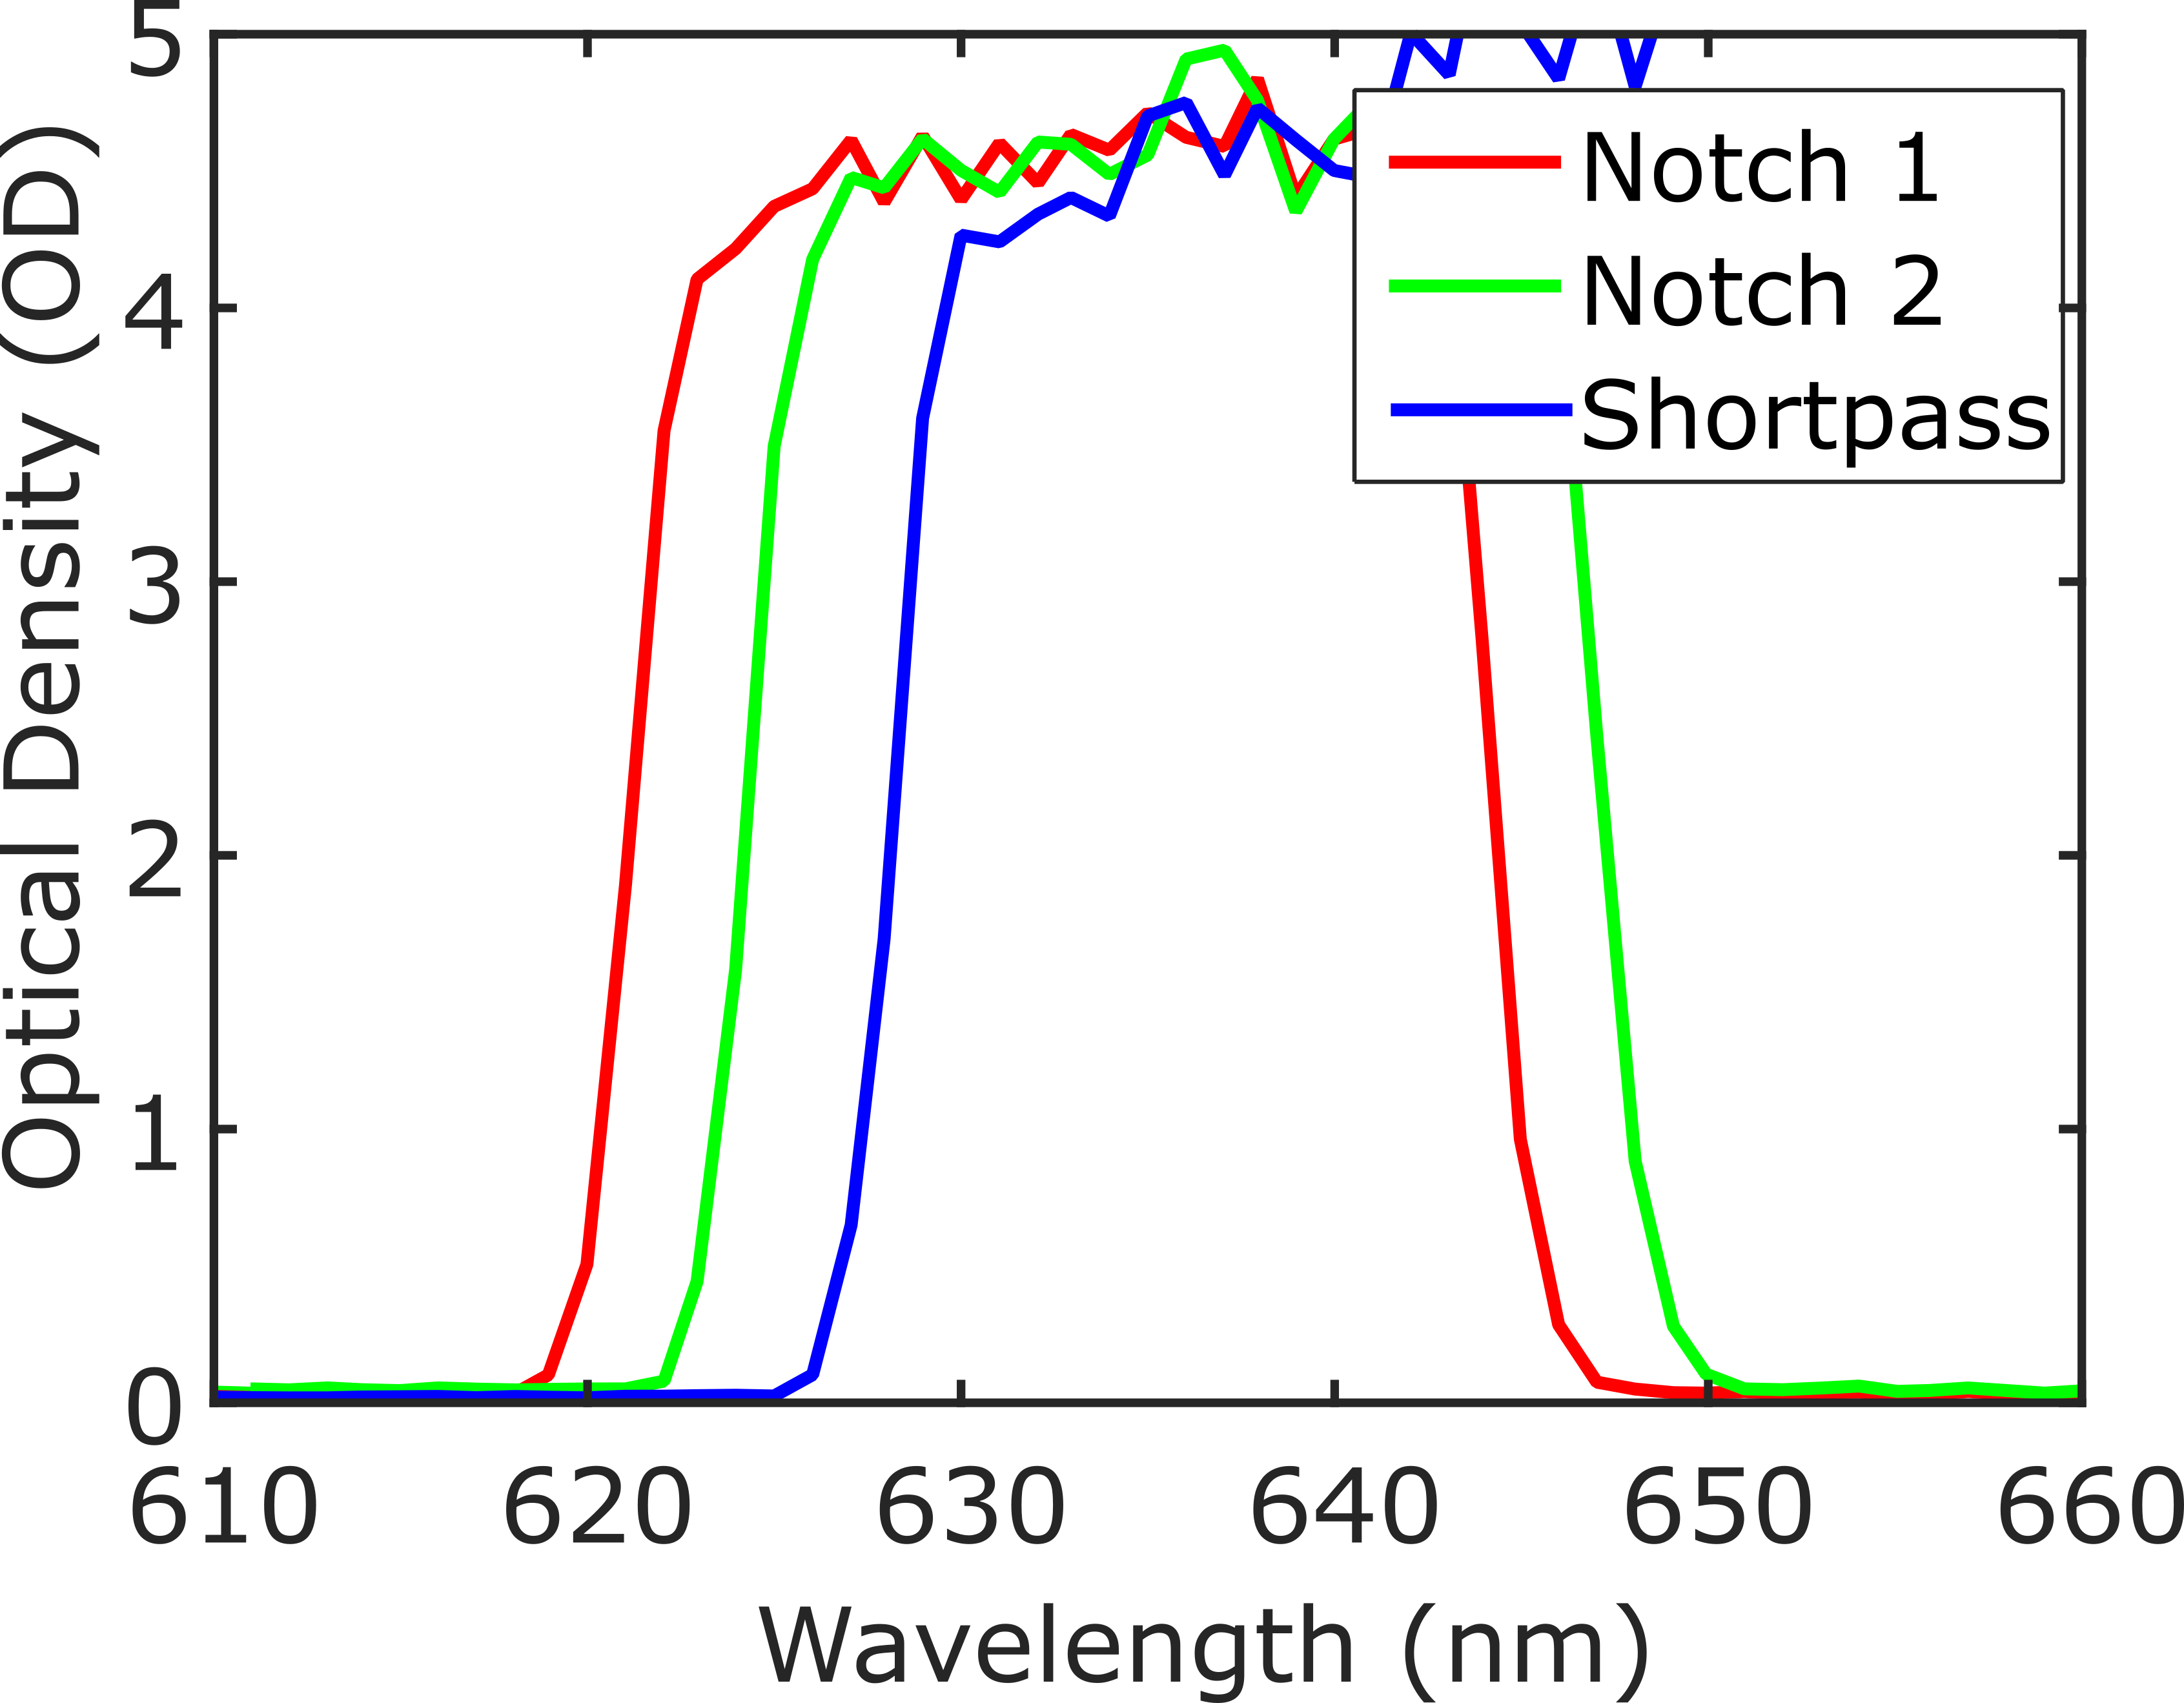
\includegraphics[width=0.45\textwidth]{Figures/Supplementary/03_Filters/filters.png}
 \caption{Normalized absorption spectrum of two notch filters and a short pass
 filter (Semrock). The normalized anti-Stokes luminescence is also displayed to
 show the effect the filters have in the total signal acquired.}
 \label{fig:filters}
 \end{figure}
 
The selection of filters play a crucial role in the signal acquired. Since the
majority of the anti-Stokes emission is concentrated around the excitation
wavelength, it is important to select filters that have a high transmission
close to the laser line. Figure \ref{fig:filters} shows the normalized
absorption spectrum of two notch filters and a short pass. Both notch are
branded as $\textrm{NF}03-633\textrm{E}-25$ but show a slightly different
absorption spectrum, shifted roughly $4\nm$ from each other. The shortpass
filter (branded as $\textrm{SP}01-633\textrm{RU}-25$) shows the transition to
transmission even closer to the laser line. 

For many fluorescence applications the exact shape of the transmission
spectrum of the filters does not play a crucial role. However for anti-Stokes
imaging, since the shape of the emission is exponential-like, this minute
changes have a great impact in the signal collected. For example, changing from
a detection path with a spectrum like notch $1$ to one like shortpass (i.e.
shifting in about $7\nm$ the edge of the filter) increases the collected number
of photons in about $50\%$. 

In this work, since only one filter does not provide enough attenuation care was
taken to always employ the notch with the most favorable transmission spectrum
in combination with either a shortpass or a longpass filter. Ideally, two
shortpass filters would have been the best solution.
 
 \section{TEM Images of rods}
 
\begin{figure}[htp]
 \centering
 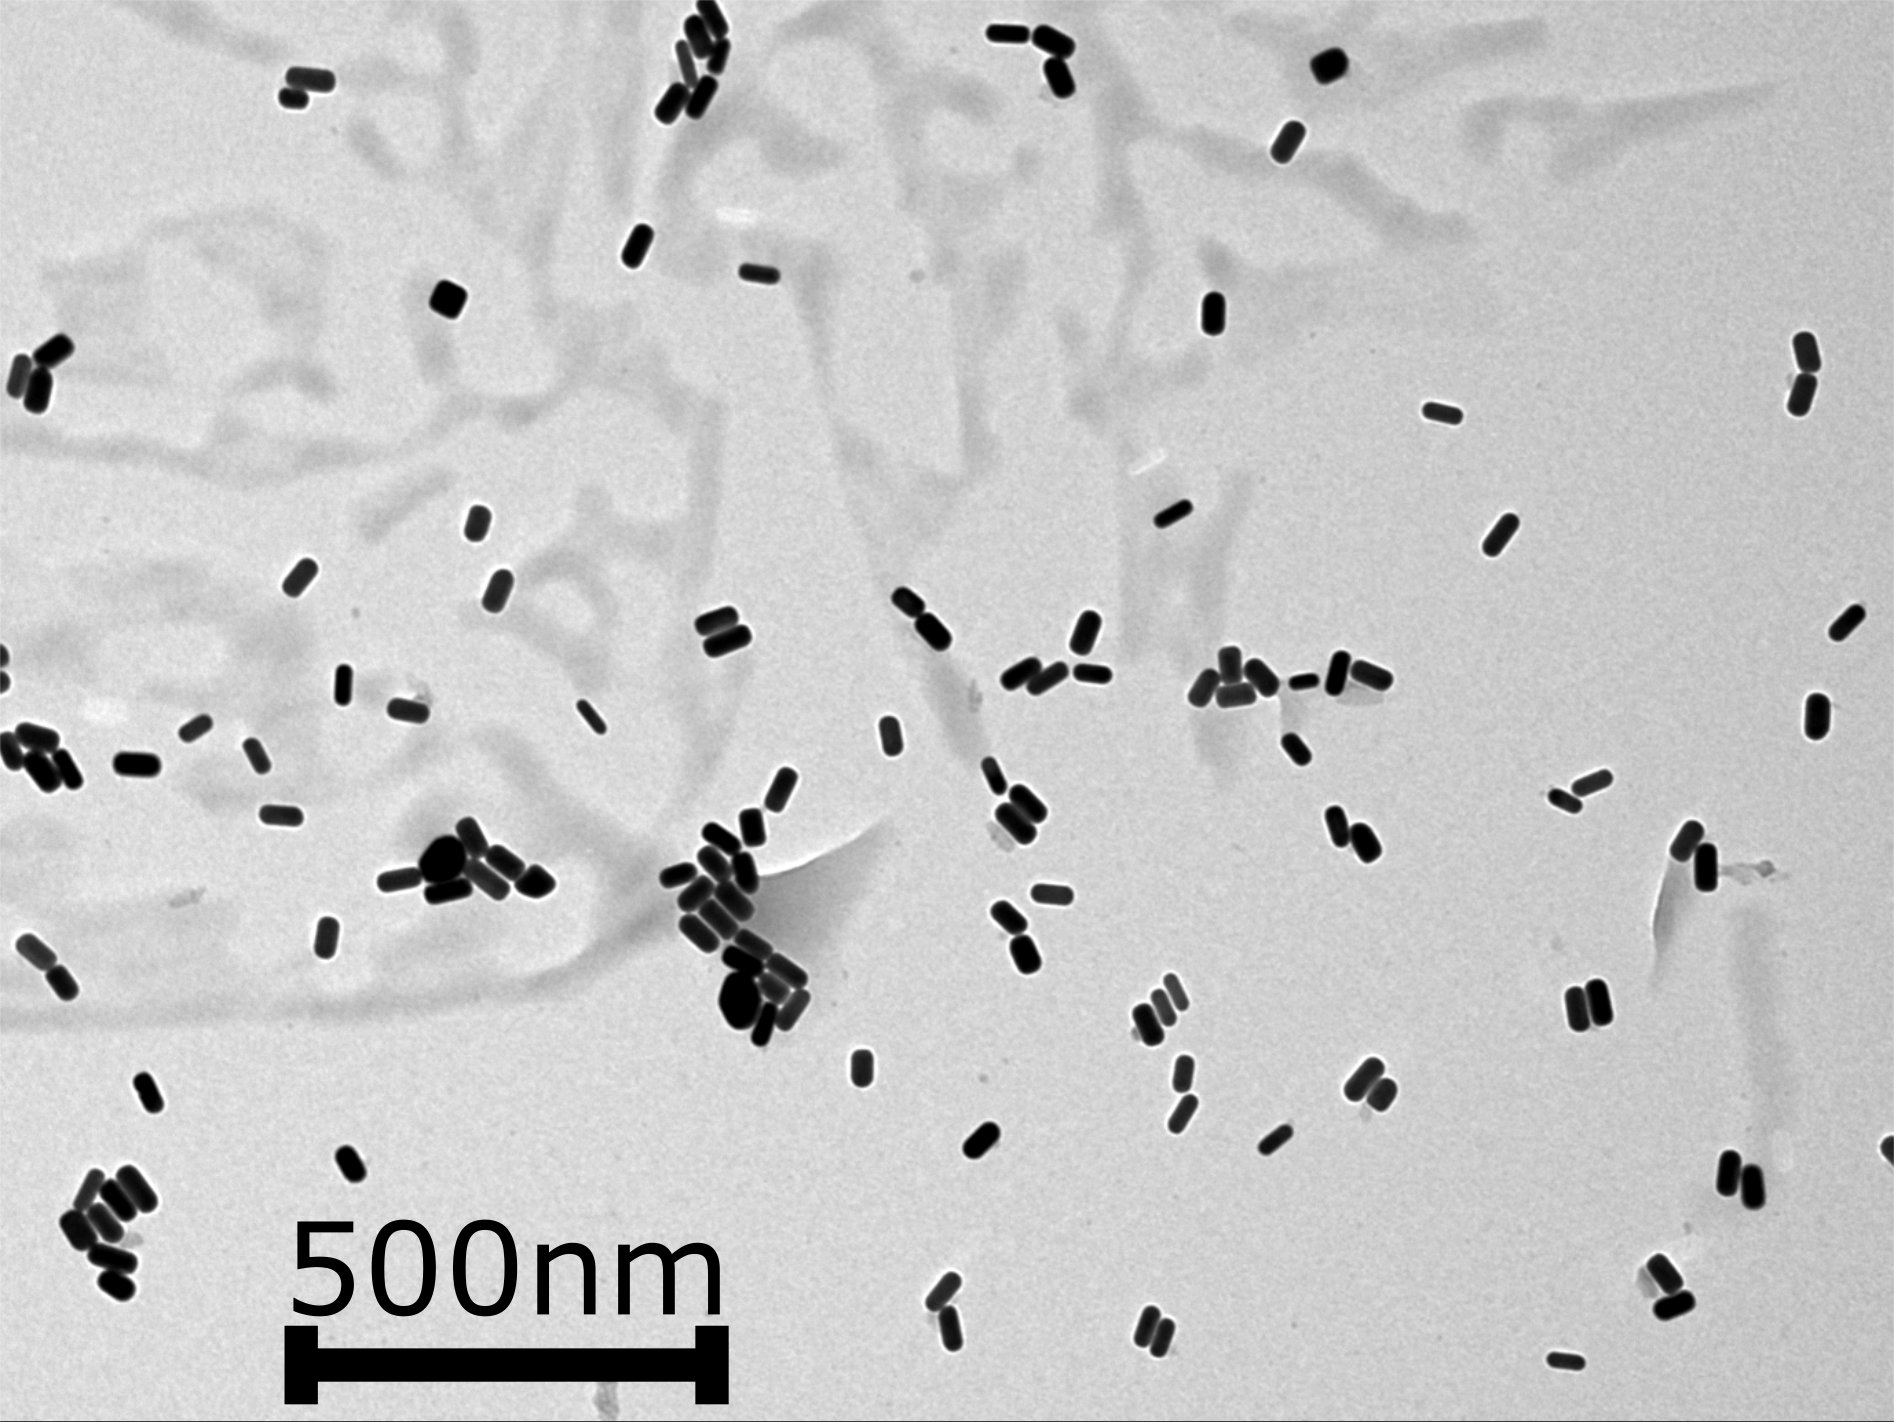
\includegraphics[width=0.45\textwidth]{Figures/Supplementary/04_TEM/tem.png}
 \caption{TEM image of the nanorod sample. The scale bar is $500\um$. }
 \label{fig:TEM}
 \end{figure}
 
Figure \ref{fig:TEM} shows an example TEM image of the gold nanorod sample.
Analysis on the dimensions of the particles yield an average length of $50\nm$
and diameter of $23\nm$. This is consistent with the plasmon observed in fig.
\ref{fig:uvvis} and at a single-particle level as in fig. \ref{fig:setup}c.

\section{White light transmission}
\begin{figure}[htp]
\centering
	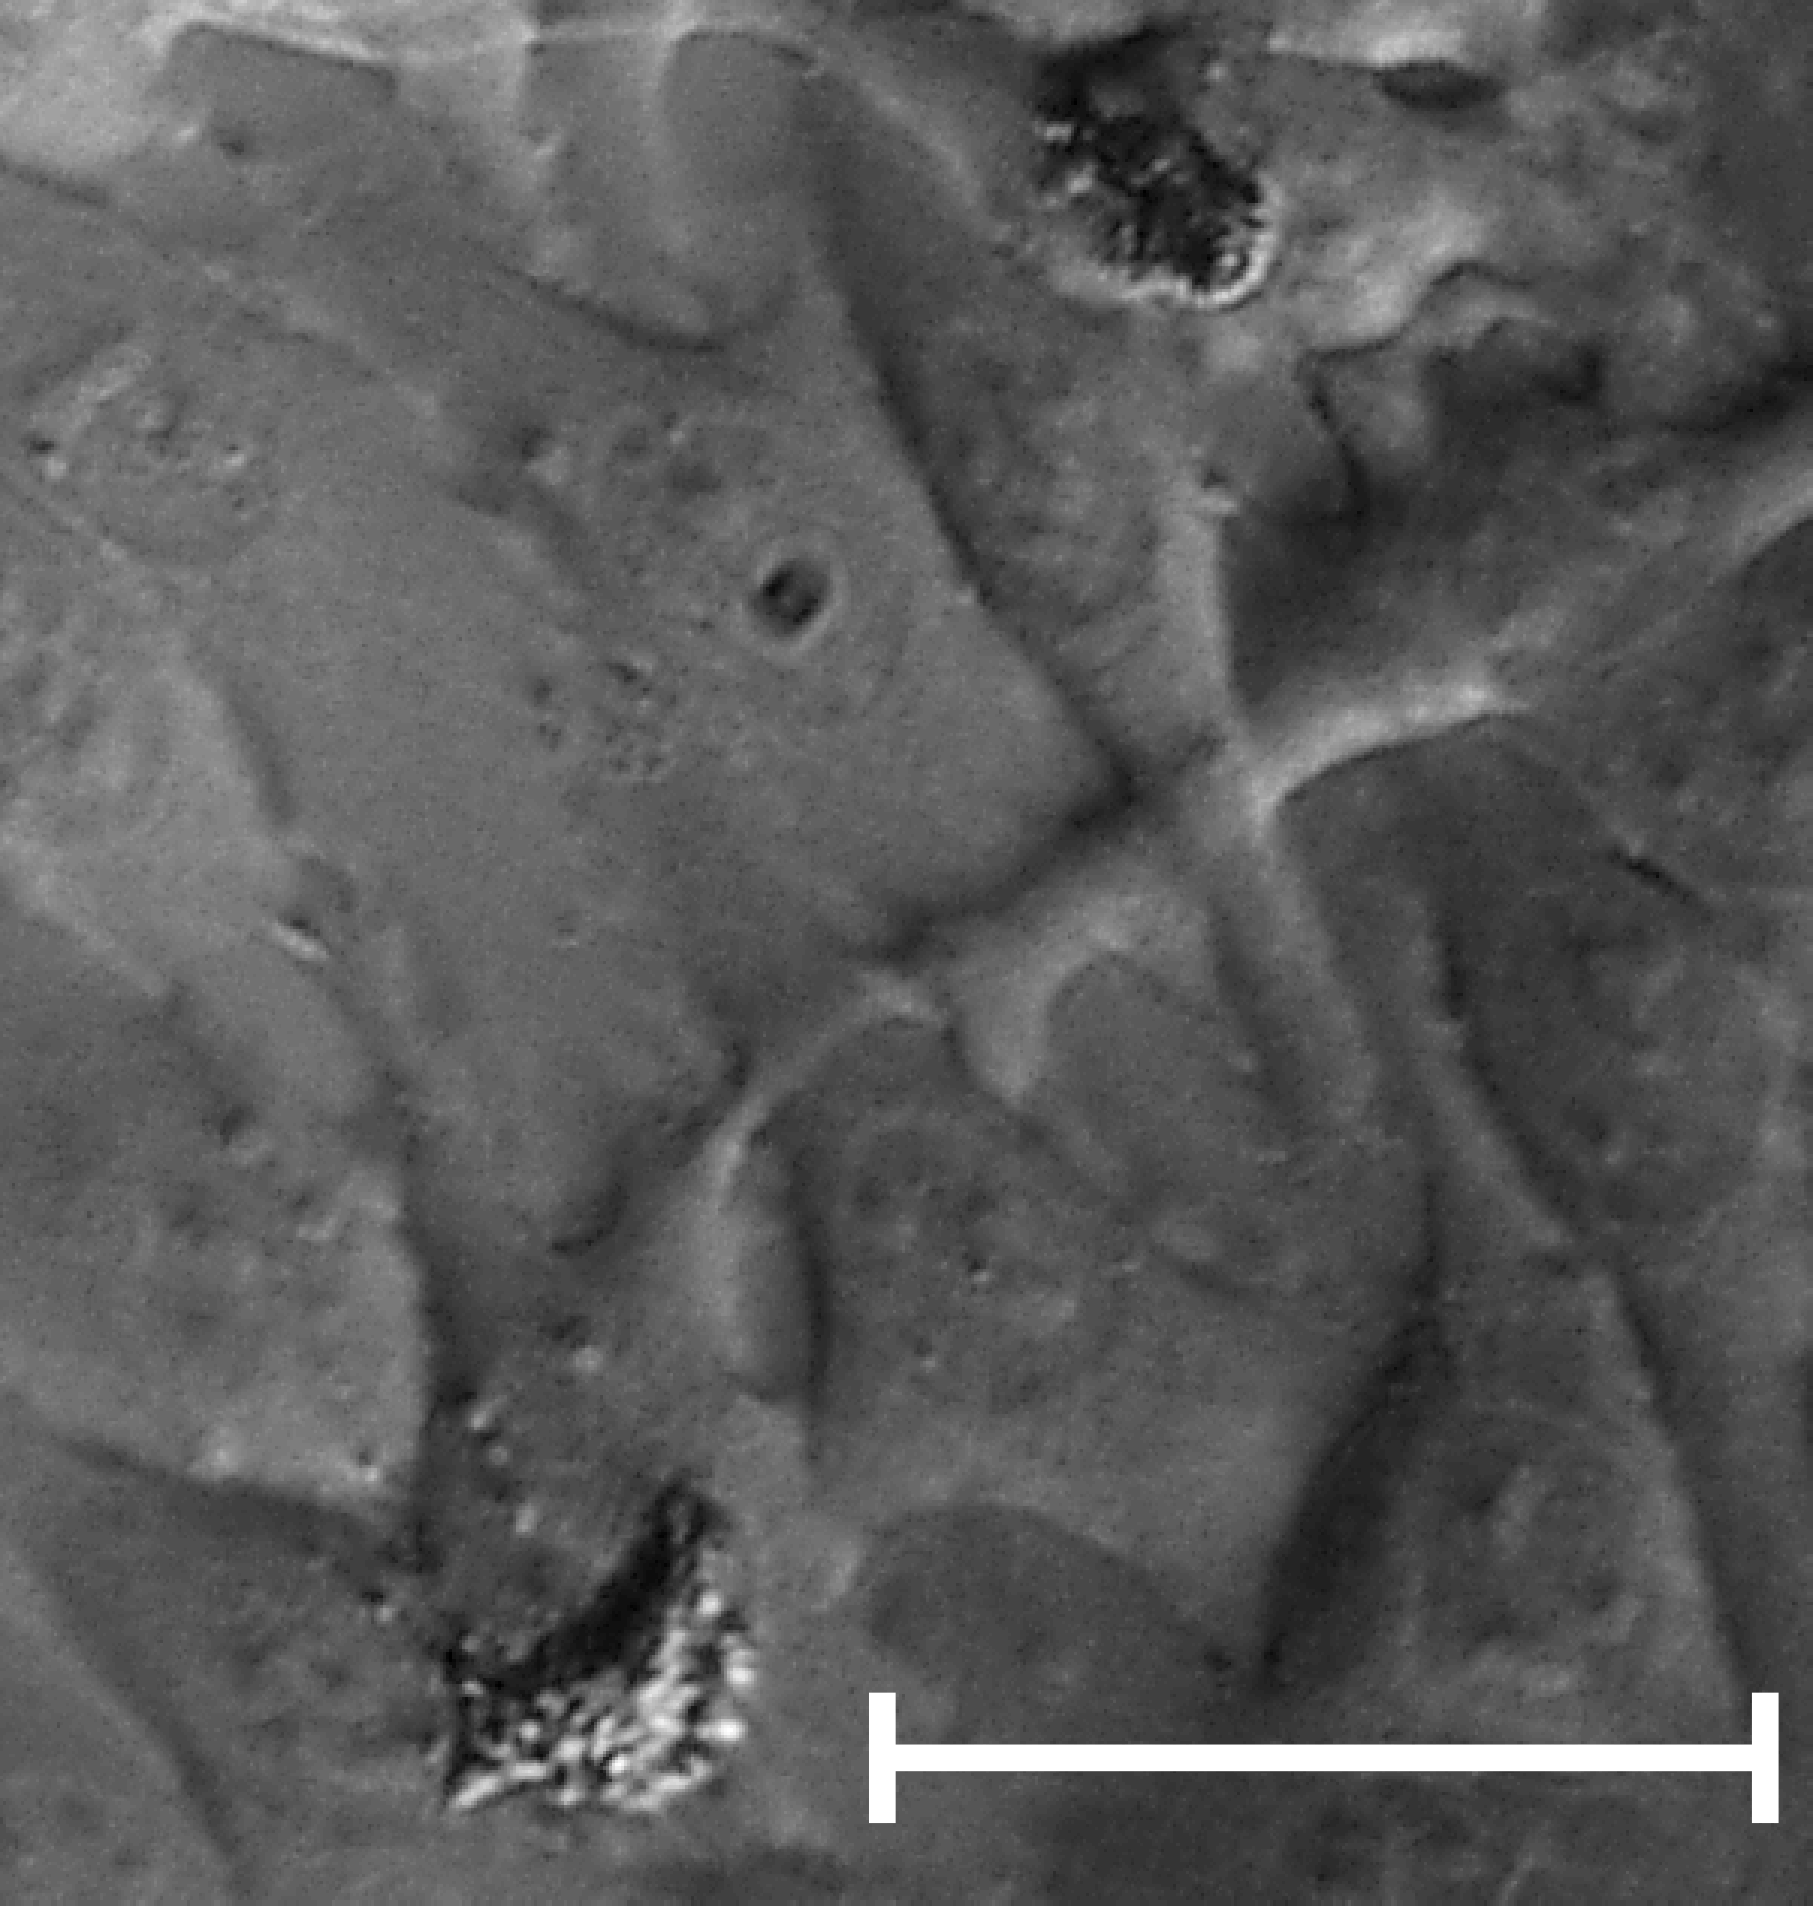
\includegraphics[width=0.45\textwidth]{Figures/Supplementary/05_White_Light/white_light_scale.png}
	\caption{White light transmission image of the sample with cells deposited on
	top of the rods. It is possible to observe that they cover entirely the
	observed region without spacing in between them. The scale bar in the figure
	is $20\um$ in length.}
	\label{fig:white-light}
\end{figure}

\end{document}